%%%%%%%%%%%%%%%%%%%%%%%%%%%%%%%%%%%%%%%%%%%%%%%%%%%%%%%%%%%%%%%%%%%%%%%%%%%%%%%%%%%%%%%%%%%%%%%%%%%%%
%
%   Version     : 2.0
%
%   Filename    : main.tex
%
%   Description : This is the main file for the LaTeX thesis proposal document template.
%                 The template is intended for use by MSCS students. 
%
%                It is assumed that you can learn how to use LaTeX on your own.
%                Please check/read the following online LaTeX book:
%
%                                 http://en.wikibooks.org/wiki/LaTeX
%     
%   Author      : Florante R. Salvador
%
%   Contributors: 1.  Karlo Campos 
%                     a. margin settings for DLSU thesis paper 
%   
%   Notes       : Please email florante.salvador@dlsu.edu.ph for comments, suggestions, ideas etc.
%
%   Reference:
%
%
%   History/Updates:
%      March 12, 2009 -- created version 1.0 for release to CSC701M (Methods of Research) students
%      May 30, 2009   -- updated Title page and Abstract for undergrad ST students
%
%      Feb 27, 2015 -- Created Version 2 (major overhaul): changed class to report, created a figures folder, 
%                               removed unnecessary packages, added new comments  based on Ethel Ong's slides
%
%%%%%%%%%%%%%%%%%%%%%%%%%%%%%%%%%%%%%%%%%%%%%%%%%%%%%%%%%%%%%%%%%%%%%%%%%%%%%%%%%%%%%%%%%%%%%%%%%%%%%%

%%%%%%%%%%%%%%%%%%%%%%%%%%%%%%%%%%%%%%%%%%%%%%%%%%%%%%%%%%%%%%%%%%%%%%%%%%%%%%%%%%%%%%%%%%%%%%%%%%%%%%%%%%%%%%%%%%%%%%%
%
%  Filename   : preamble.tex
%
%  Description: Preamble file to :
%               a. specify related packages
%               b. set margins, commands, etc.
%
%  Note       : Edit the margin settings for your own printer
%                  You may add your own commands, environments (it is assumed that you know what you're doing.)
%
%%%%%%%%%%%%%%%%%%%%%%%%%%%%%%%%%%%%%%%%%%%%%%%%%%%%%%%%%%%%%%%%%%%%%%%%%%%%%%%%%%%%%%%%%%%%%%%%%%%%%%%%%%%%%%%%%%%%%%%

%\documentclass[12pt,titlepage,onepage, letterpaper]{article}

\documentclass[12pt,titlepage,onepage, letterpaper]{report}


%
%-- specify related packages
%

%
% \usepackage[utf8x]{inputenc}
%

\usepackage{apacite}           %-- APA style citation 
                               %-- refer to http://www.ctan.org/tex-archive/biblio/bibtex/contrib/apacite/

%
%  \usepackage{ucs}
%


\usepackage{amsmath}           %-- American Math Society packages
\usepackage{amsfonts}
\usepackage{amssymb}


\usepackage{graphicx}          %-- graphicx package needed for including figures in JPG or PNG format
 
%
%\usepackage{graphics}          %-- graphics related package (this was commented out) use when image is in EPS format
%

\usepackage{verbatim}          %-- this package allows you to have multiple lines of comments by
                               %-- example:
                               %   \begin{comment}
                               %        ...your text here...
                               %   \end{comment}  

\usepackage{color}             %-- allows use of color with text
                               %-- example:  \textcolor{red}{This is the colored text in red.}

\usepackage{url}  %-- allows use of URLs example: \url{https:\ccs1.dlsu.edu.ph}

%% MY ADDED PACKAGES
\usepackage[export]{adjustbox}          %-- This is for setting max size in figure width
\usepackage[space]{grffile}             %-- This allows spaces in filenames
\usepackage{mathtools}                  %-- For left-align of matrix elements
\usepackage{booktabs}                   %-- For complicated tables
\usepackage{multirow}                   %-- For complicated tables
\usepackage{colortbl}                   %-- For table border
\usepackage{vcell}                      %-- For top alignment of cells
\usepackage{tabularx}                   %-- For autofit table (ex. begin{tabularx}{\columnwidth}{X|X})
%%%%%%%%%%%%%%%%%%%%%%%%%%%%%%%%
%
%-- set margins,  you may need to edit this for your own printer
%
\topmargin 0.0in
\oddsidemargin 0.0in
\evensidemargin 0.0in

\voffset 0.0in
\hoffset 0.5625in

\textwidth 5.75in
\textheight 8.5in


\parskip 1em
\parindent 0.25in

\bibliographystyle{apacite}            %-- use APA citation scheme

\hyphenation{ana-lysis know-ledge}     %-- LaTeX may not hyphenate correctly some words you use in your document
                                       %-- use \hyphenation to instruct LaTeX how to do it correctly, example above

\newcommand{\degree}{^{\circ}}         %-- use \newcommand to create your own "commands"
                                       %-- \newcommand works like the #define you learned in your COMPRO1 class

\newcommand{\etal}{et al.}


%\newcommand{\sinag}{\emph{Sinag}}
%\newcommand{\sinagtwo}{\emph{Sinag2}}

\newcommand{\figref}[1]{Figure \ref{#1}}
\newcommand{\appref}[1]{Appendix \ref{#1}}

%-- \newcommand{\Section}[1]{\section{#1}\setcounter{figure}{0}\setcounter{table}{0}}

%\newcommand{\shade}{\multicolumn{1}{|>{\columncolor[gray]{0.25}}c|}{}}
%\newcommand{\tableheader}[1]{\rowcolor{black}\color{white}{#1}}
%\newcommand{\cell}[2]{\multicolumn{1}{#1}{#2}}
%\newcommand{\definition}[2]{\textbf{\textit{#1}} --- #2}
%\newcommand{\itembit}[1]{\item \textbf{\textit{#1}}}
%\newcommand{\sgdef}[2]{\parbox[t][][t]{1.75in}{\textbf{#1}} \> \parbox[t][][t]{4.0in}{#2}\\\\}

%\newenvironment{sinagglossary}{\begin{flushleft}
%\begin{tabbing}
%\hspace{1.75in}\=\\}{\end{tabbing}\end{flushleft}}

\newcommand{\thestitle}[1]{{\Large \textsc{#1}}}


%---
%  \renewcommand{\thefigure}{\thesection.\arabic{figure}}
%  \renewcommand{\thetable}{\thesection.\arabic{table}}
%  \renewcommand{\contentsname}{Table of Contents}




                %-- includes LaTeX source file for the preamble 
                                  %-- include packages, sets the margin sequence, and many more... 
                                  %-- your job: check if the settings are suitable for your own printer

\graphicspath{{figures/}}  %-- figures is the name of the folder containing images JPG or PN

\begin{document}

%%%%%%%%%%%%%%%%%%%%%%%%%%%%%%%%%%%%%%%%%%%%%%%%%%%%%%%%%%%%%%%%%%%%%%%%%%%%%%%%%%%%%%%%%%%%%%%%%%%%%%
%
%   Filename    : title_page.tex 
%
%   Description : This file will contain your Title Page.
%                 
%%%%%%%%%%%%%%%%%%%%%%%%%%%%%%%%%%%%%%%%%%%%%%%%%%%%%%%%%%%%%%%%%%%%%%%%%%%%%%%%%%%%%%%%%%%%%%%%%%%%%%

\begin{titlepage}
\centering


%-- **EDIT** the following line to indicate your thesis title
\thestitle{Model-Based Clustering of Digital PCR Droplets using Expectation Maximization}

\vspace{1.75cm}
A Thesis Proposal\\
Presented to\\
the Faculty of the College of Science\\
De La Salle University Manila

\vspace{1.75cm}
In Partial Fulfillment\\
of the Requirements for the Degree of\\
Master of Science in Statistics

\vspace{1.75cm}
by\\
%-- **EDIT** the following line to indicate your name 
\vspace{1cm}

GUIAO, Joyce Emlyn B.  \\

%LASTNAME2, FirstName2  \\
%LASTNAME3, FirstName3  \\
% LASTNAME4, FirstName4  \\

% \vspace{1.75cm}
% %-- **EDIT** the following line to indicate your adviser's name 
% Frumencio F. Co \\
% Adviser

\vspace{1.75cm}
\today
\end{titlepage}
              %-- includes LaTeX source file for the Title Page 
                                  %-- your job: **EDIT THIS FILE ** to indicate your own title, name, and thesis adviser's name


%%%%%%%%%%%%%%%%%%%%%%%%%%%%%%%%%%%%%%%%%%%%%%%%%%%%%%%%%%%%%%%%%%%%%%%%%%%%%%%%%%%%%%%%%%%%%%%%%%%%%%
%
%   Filename    : abstract.tex 
%
%   Description : This file will contain your abstract.
%                 
%%%%%%%%%%%%%%%%%%%%%%%%%%%%%%%%%%%%%%%%%%%%%%%%%%%%%%%%%%%%%%%%%%%%%%%%%%%%%%%%%%%%%%%%%%%%%%%%%%%%%%

\begin{abstract}
The digital PCR (dPCR) is a method to quantify the DNA copies of known strains related to diseases. As a new approach to the gold-standard RT-PCR, further research is required to assess the quality and accuracy of this method. One particular area of dPCR is its novel step in droplet classification that distinguishes it from RT-PCR. As of writing, few droplet classifiers exist in literature as well as the assessment of these methods. This thesis reviews the classification methods of current dPCR quantification tools in literature, and proposes the Expectation Maximization Clustering method in aims to improve the accuracy of the final estimated DNA concentration.

%
%  Do not put citations or quotes in the abract.
%

\begin{flushleft}
\begin{tabular}{lp{4.25in}}
\hspace{-0.5em}\textbf{Keywords:}\hspace{0.25em} & Quantitative PCR, Droplet Digital PCR, Expectation Maximization Clustering \\
\end{tabular}
\end{flushleft}
\end{abstract}
                %-- this is the Abstract page
                                  %-- your job: **EDIT THIS FILE** to indicate your own abstract

\pagenumbering{roman}             %-- this will number pages as i, ii, iii, etc...
\setcounter{page}{2}

\tableofcontents                  %-- this command is used to generate the Table of Contents


\newpage
\listoffigures                    %-- this command is used to generate List of Figures

\newpage                       
\listoftables                     %-- this command is used to generate List of Tables

\newpage

\pagenumbering{arabic}            %-- this will number pages as 1, 2, 3, etc...
\setcounter{page}{1}              


\chapter{Research Description}
\label{sec:researchdesc} 

\section{Introduction}
\label{sec:introduction}

\section{Background of the Study}
\label{sec:backgroundstudy}

% What is NA Quantification and its applications ? %
Quantification of Nucleic acids (NA) is a developing research field in molecular biology for the detection and quantification expression levels of genes \cite{Huggett2015}. These NA molecules are found in deoxyribonucleic acid (DNA) and ribonucleic acid (RNA), which carries genetic information and is used as biomarkers for the detection of diseases. Additionally, along with the rise of bioinformatics tools, NA quantification methods are also utilized in rare mutation detection, copy number variation detection, single-cell gene and microRNA expression analysis, and next-generation sequencing \cite{Quan2018}. Outside the scope of molecular biology, its application has also found its way in forensic research \cite{Whale2013}, medical diagnosis, environmental monitoring, and food safety analysis \cite{Cao2017}.


% How to Quantify NA Quantification with (dPRC) ? %
To be able to determine the concentration of target NAs, NA detection is naturally a pre-requisite. There are, however, NAs of interests that have very low concentrations to the point that it becomes undetectable in existing detection technologies. This problem is solved by amplifying the NA sequences using Polymerase Chain Reaction (PCR), a widely-used method for NA amplification since its invention in the 1980s \cite{Cao2017}. PCR can multiply specific NA sequences in DNA or RNA from low concentrations to millions of copies. This method exposes the NA sequences mixed with chemical components in a series of 20 to 40 temperature cycles. In each cycle, PCR doubles the NA molecule; theoretically producing \(2^n\) molecules after \(n\) cycles \cite{Quan2018}.

After PCR amplification, absolute NA quantification is achieved using digital Polymerase Chain Reaction (dPCR) technique. This equally divides the NA samples into thousands of partitions; each of these partitions is evaluated as either off or on, or in this context, labeled as positive or negative, hence the term "digital" \cite{Cao2017}.

The dPCR workflow, as illustrated in \figref{fig:dpcrWorkflow}, is usually a sequential procedure of extracting the sample from an organism, concocting the sample with several chemical components into a reaction mix, distributing the reaction mix to equal partitions, amplifying and detecting the target molecules using PCR, and the concentration is then finally estimated using a Poisson correction factor. In \cite{Jacobs2014}, it was emphasized that every step of the dPCR workflow inevitably allows for the introduction of different sources of variation. These variance components within the dPCR workflow is shown in \figref{fig:workflowVariation}. 

\begin{figure}[h]
    \centering
    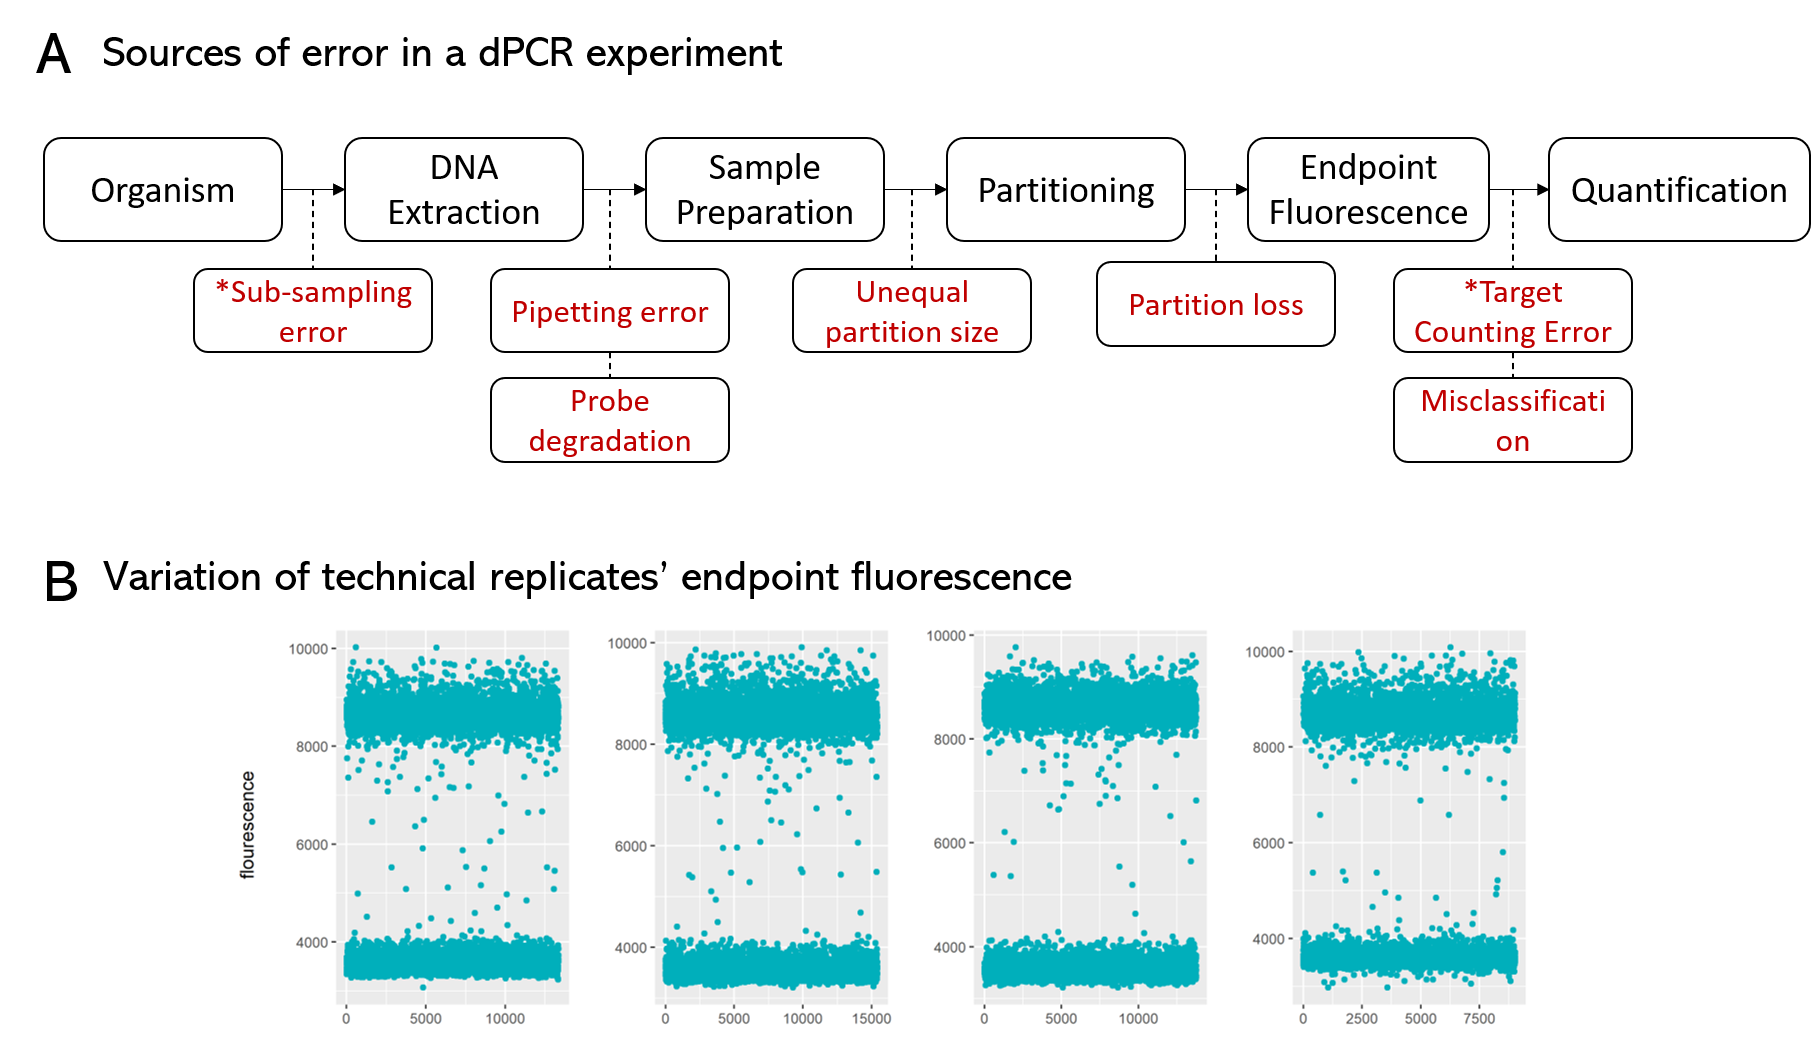
\includegraphics[max size={\textwidth}{\textheight}]{dpcrWorkflow.png}
    \caption{The dPCR workflow}
        \label{fig:dpcrWorkflow}
\end{figure}

\begin{figure}[h]
    \centering
    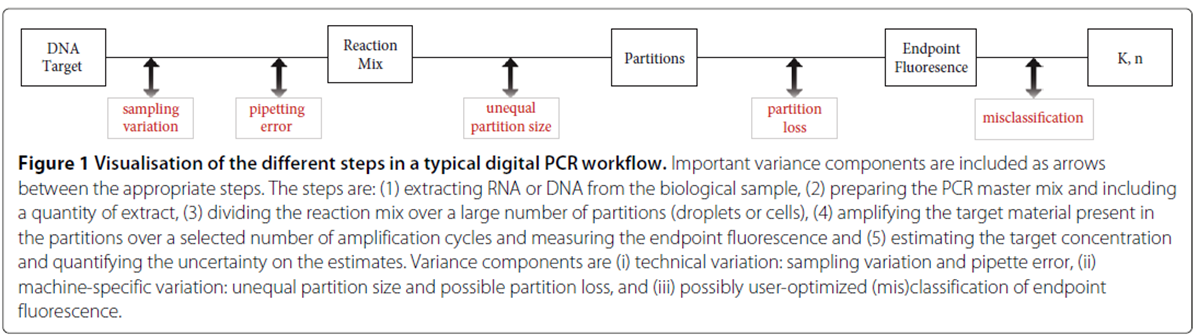
\includegraphics[max size={\textwidth}{\textheight}]{workflowVariation.png}
    \caption{Potential variation components between steps of the dPCR workflow}
        \label{fig:workflowVariation}
\end{figure}

Sampling variation stems from the fact that only a small sample of the organism is extracted; and although there is an expected number of target molecules per liters of a sample, drawing equally sized samples will result in different target molecules that are more or less near the average. \shortciteA{Tzonev} demonstrates the number of target molecules that can be drawn from extraction is distributed as Poisson. Besides the sampling error, samples may also exhibit imperfections, and thus have inhibited amplification. 

Preparing the reaction mix is a delicate process that strictly requires the accuracy of the pipetting volume; and yet, technical variation still occurs that results in pipetting errors. The next variation components are the possibility of the distributed partitions to be of unequal volumes and the loss of partitions due to physical interventions. Finally, upon PCR amplification, each droplet partition emits an endpoint fluorescence that would be used to classify the partition as positive or negative. However, some partitions are difficult to classify due to inhibition, delayed reactions, primer depletion, and other biological factors.

Each variance component accumulates to the bias and variance of the final estimated target molecule concentration, and thus, this gives rise to the importance of providing solutions that would increase precision in every step. To increase the sensitivity and specificity of the estimate, the misclassification of droplet partition should be minimized as much as possible. A high presence of false-negative droplets reduces sensitivity, while specificity is lowered for high false-positive count. Due to the variance contributed by misclassification, \shortciteA{Tzonev} recommends reporting the rates of false positives (FPR) and false negatives (FPN) per partition. More importance is given to either of the two depending on the kind of test being performed. If the total negative partition is expected to be large, then there is more chance that a true negative partition may turn into a false positive reading; which in this case, FPR may be of more interest than FNR. 

The primary problem in misclassification lies in 'rain' droplets; these are partitions that emits an intermediate fluorescence signal that is difficult to classify as positive or negative. Figures \ref{fig:plate1cru} and \ref{fig:plate1tc1507} demonstrates two different DNA targets with the former showing a visually clearer distinction of the positive and negative population than the latter, of which is possessing multiple rain droplets. The data used in these figures are sourced from the publicly available dataset from the study of \shortciteA{Lievens2016}. 

\begin{figure}[h]
    \centering
    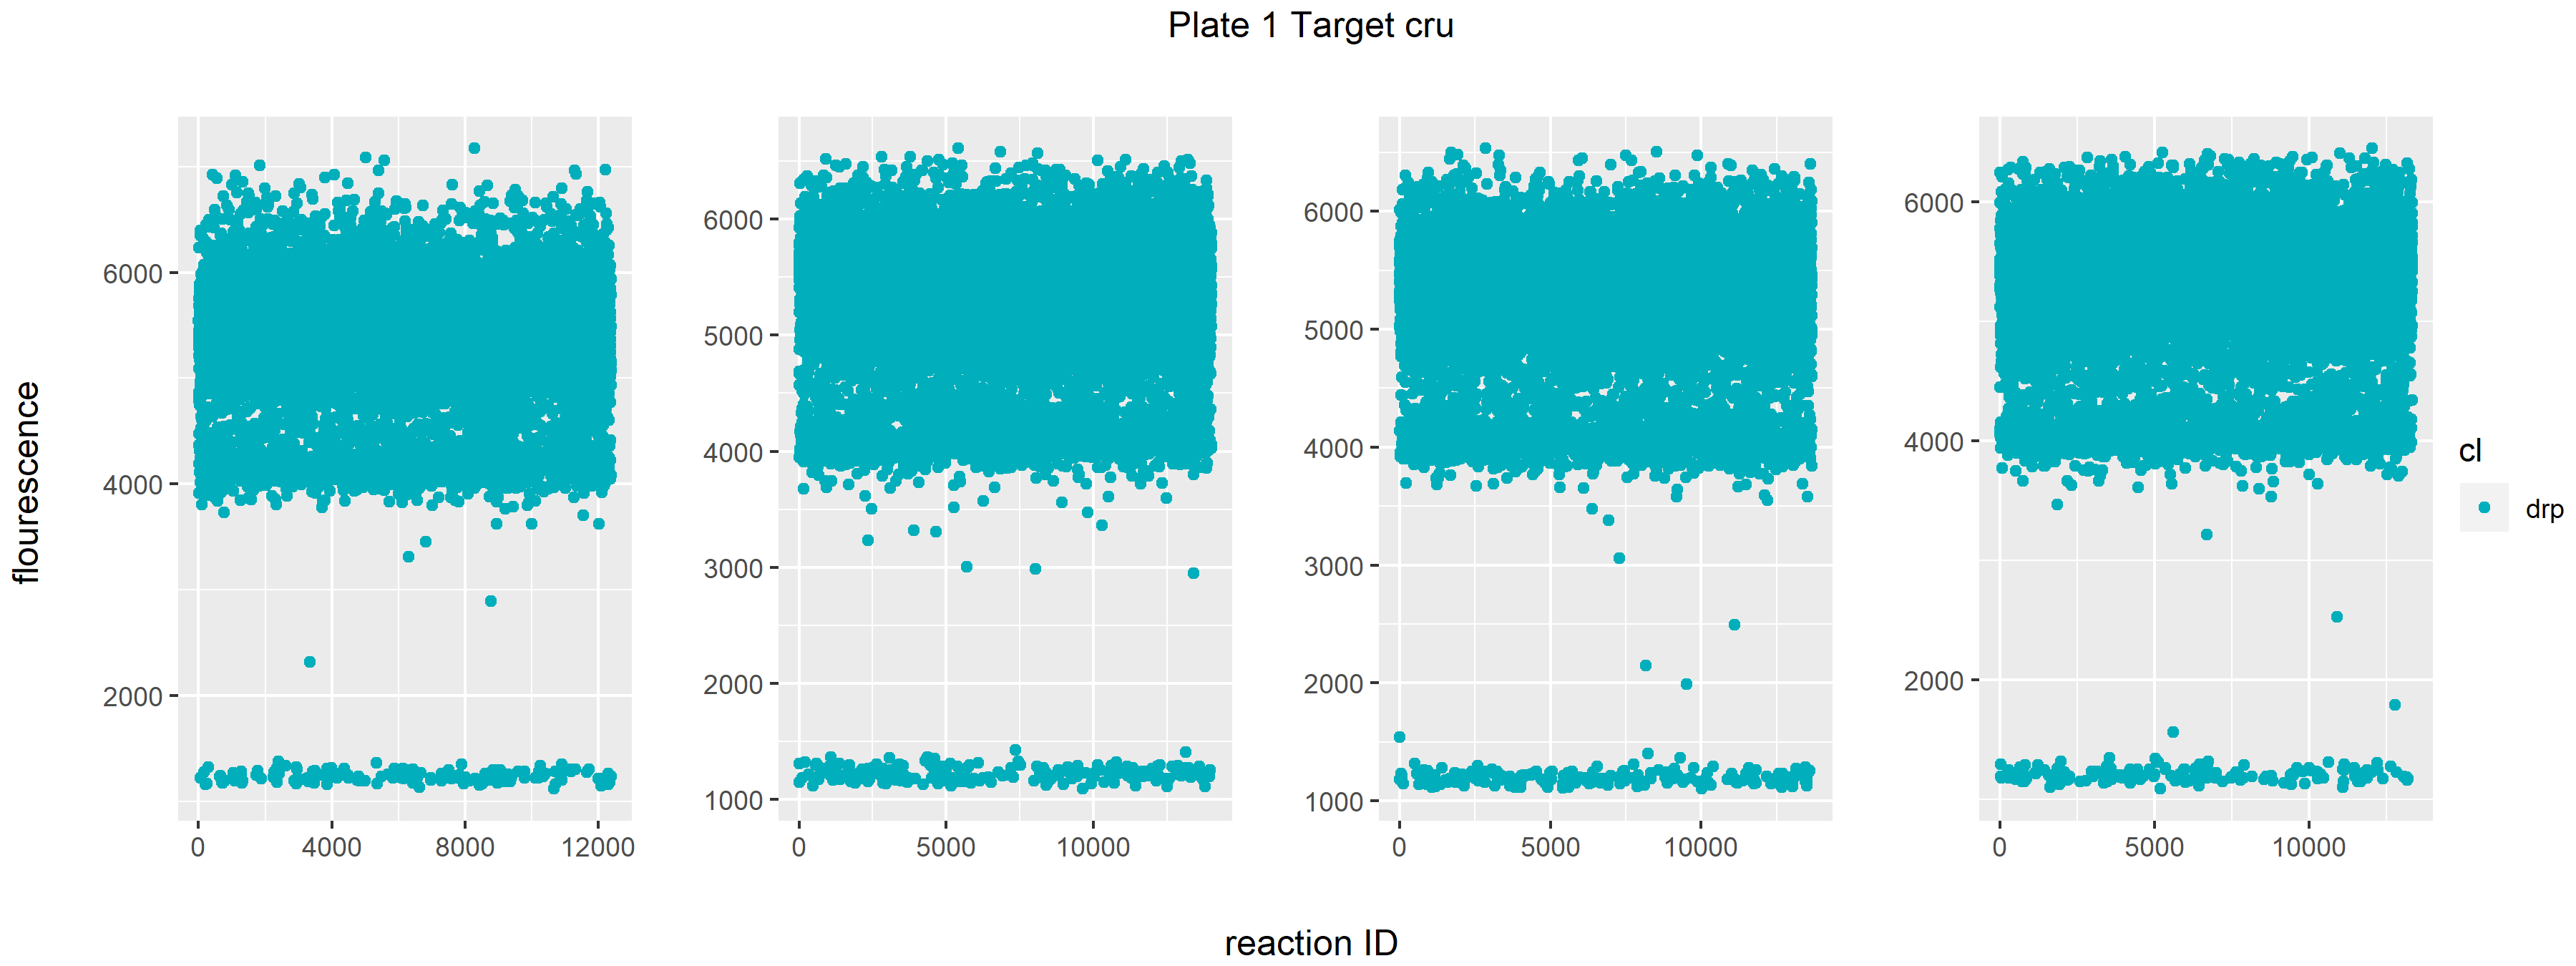
\includegraphics[max size={\textwidth}{\textheight}]{Plate 1 Target cru.png}
    \caption{Fluorescence readings of 4 repititions of DNA target cru}
        \label{fig:plate1cru}
\end{figure}

\begin{figure}[h]
    \centering
    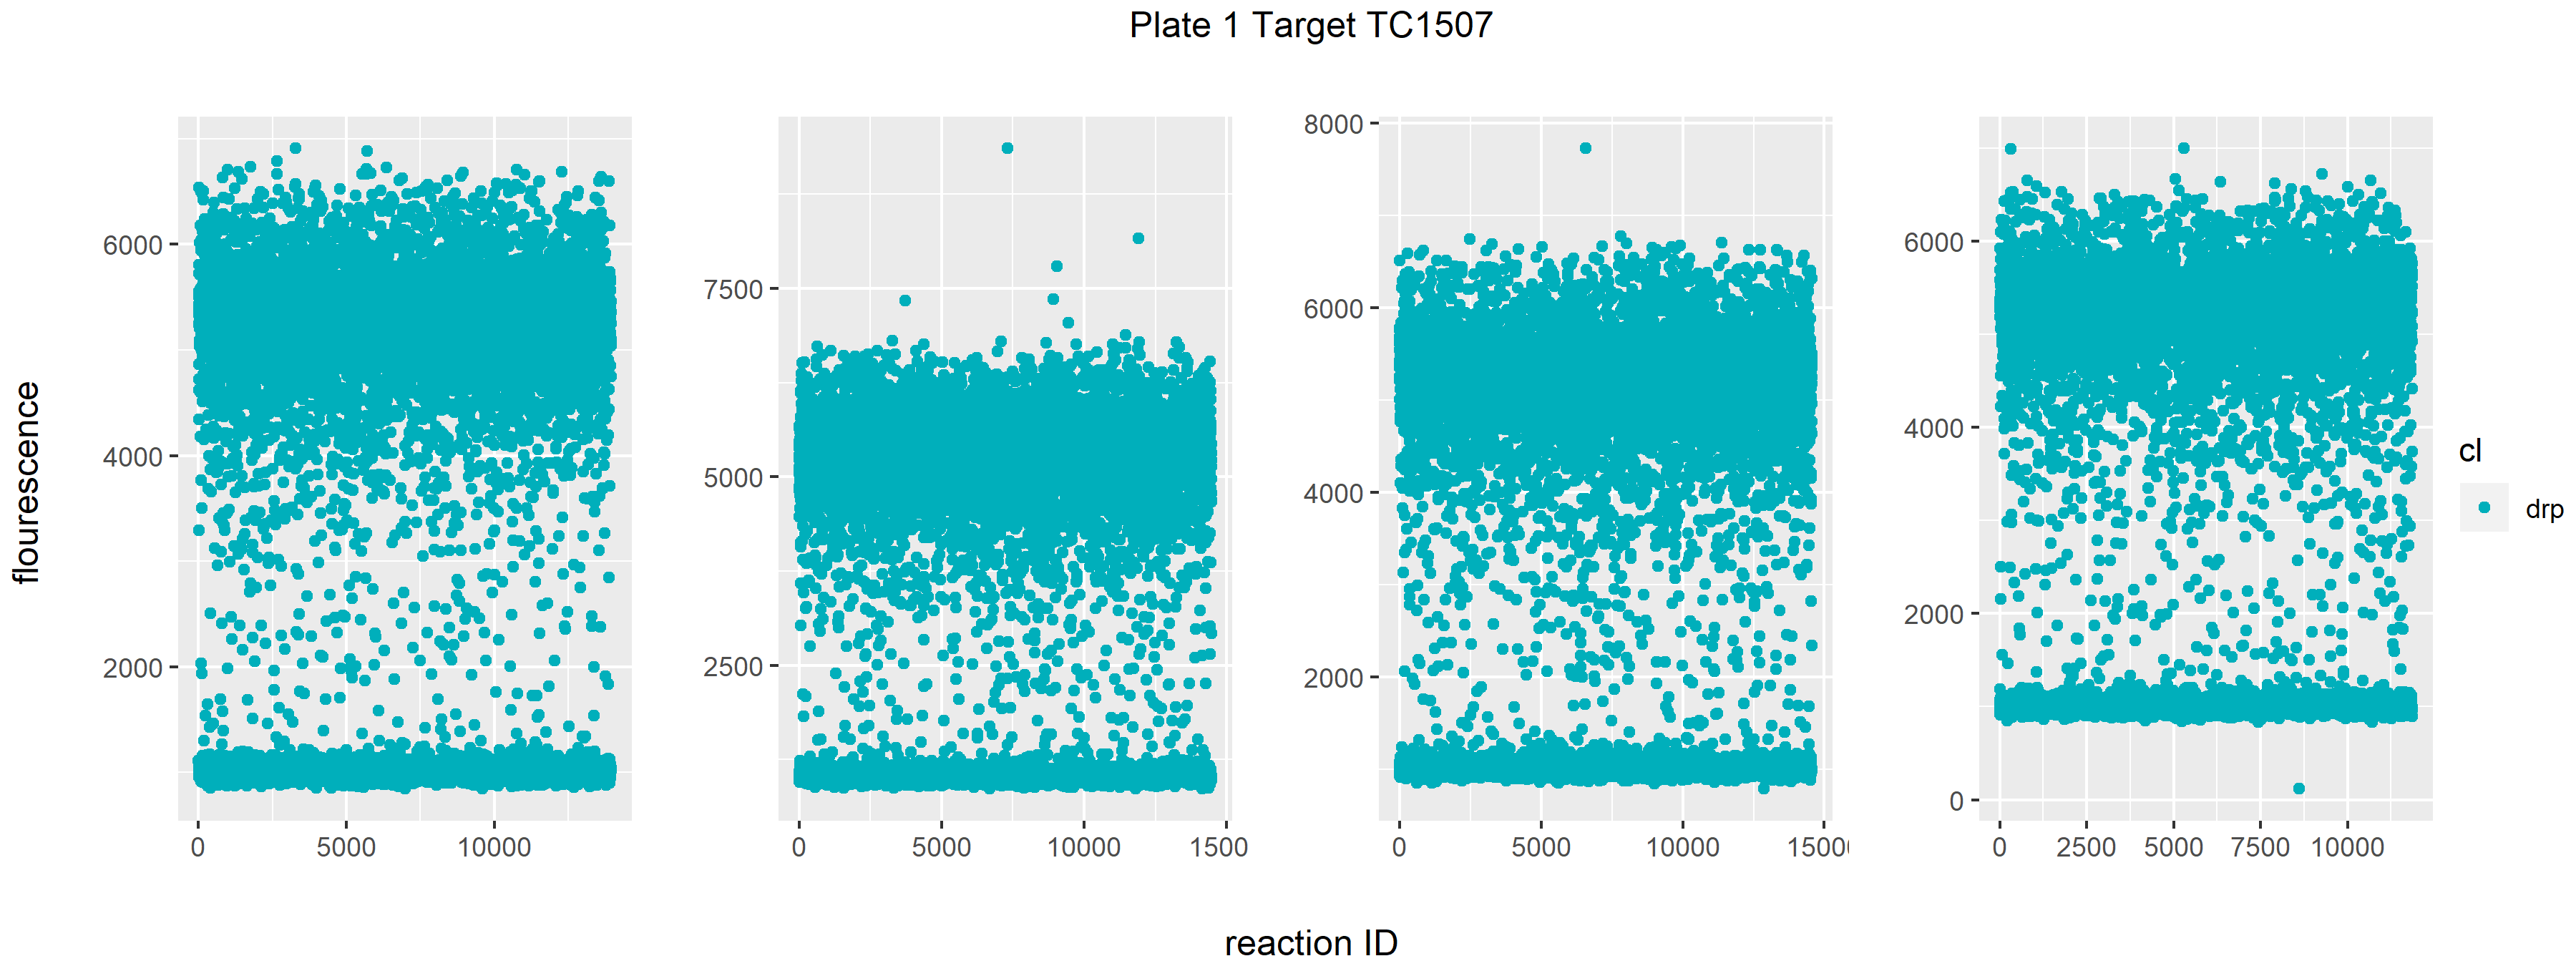
\includegraphics[max size={\textwidth}{\textheight}]{Plate 1 Target TC1507.png}
    \caption{Fluorescence readings of 4 repititions of DNA target TC1507}
        \label{fig:plate1tc1507}
\end{figure}

The estimate for DNA target concentration highly depends on the positive and negative classifications. For experiments with low copy DNA targets, the focus is on maximizing the sensitivity of the test for these very small number of positive droplets. Low sensitivity translates to failure in detecting lower concentrations. 

For assays with large differences in the distance between the two fluorescence groups (positive and negative droplets), most quantification tools estimate the target concentrations with high sensitivity. As exhibited in an optimized assay experiment of E. amylovora \cite{Dreo2014}, slight differences of thresholds calculated from different tools had little effect on the final estimated concentration. However, for R. solanacearum, which is observed to manifest false-positive signals in qPCR experiments, produces unsatisfactory analytical sensitivity of the concentration estimates. 


% \citeA{Jones2014} stresses the impact of false positives for DNA targets of low copy numbers. This is because the count of false positive droplets will highly influence the relative proportion of total positive droplets. %

The danger of false rates due to misclassification is expounded at the clinical level, where false rates lead to the misdiagnosis of patients \cite{Tzonev}. One such case is the prenatal screening test for Down Syndrome; this test is expected to mostly result in normal pregnancies. However, even for a small FPR, many pregnancies are still falsely reported as positive for Down Syndrome. False negatives also risk the overall health of the patient that truly possesses the genetic disorder.




\section{Statement of the Problem}
\label{sec:statementprob}

This thesis aims to classify dPCR droplet partitions into positive or negative by exploring Model-Based clustering with Expectation Maximization. The specific objectives of this study are to:
\begin{enumerate}
    \item Fit two-component finite mixture densities on the datasets with varying amounts of rain and increasing target DNA concentration;
    \item Classify partitions using the fitted models for each experiment and estimate DNA concentration using the standard formula;
    \item Evaluate and compare the precision and bias of the estimates amongst the existing classification methods. 
\end{enumerate}

\section{Significance of the Study}
\label{sec:significancestudy}
Quantification of target concentrations for pathogenic bacteria, gene expression of diseases, cancer diagnostic, and other health-related applications strongly demand estimators with high sensitivity and precision, as lives are put to risk for false-positives. A modern approach to DNA and RNA target quantification is through the dPCR method. In one of the steps of the dPCR workflow, the classification of droplet fluorescence still has areas of improvement. 

The most prominent problem in classification lies in experiments exhibiting a high frequency of rain, or intermediate fluorescence values. These are experiments that have not yet been optimized. As different DNA target samples exhibit distinct structures \cite{Lievens2016}, an optimized setup for one DNA target may not be applicable for other targets. Additionally, for samples with low concentration, the total count of detected positive droplets dramatically changes the final concentration estimate, due to the greater impact of false positives in the proportion of detected over the number of true positives. The following are some tools and methodologies proposed for droplet classification: Quantasoft propriety software, definetherain \cite{Jones2014}, manual global threshold \cite{Dreo2014}, cloudy \cite{Lievens2016}, and Umbrella \cite{Jacobs2017}. Most of the aforementioned droplet classifying tools rely strongly on how representative reference samples are. According to \citeA{Dreo2014}, such approaches are sensitive to significant shifts in amplitude for previously unobserved factors, such as cross-reactions or the influence of inhibitors.

In an attempt to prevent the problem of representation, this study will explore the feasibility of estimating target concentrations without a reference sample. Similar to Umbrella, this study also aims to use model-based clustering for the droplet classification but with relaxing the assumptions using the Expectation-Maximization algorithm. The significance of the study will be useful in quantifying concentrations in targets that have not yet been optimized for dPCR experiments and also for quantifying targets of low concentrations. 

\section{Scope and Limitations}
\label{sec:significance}
This study solely relied on publicly available fluorescence datasets from published research papers. Only two were found and will be used for statistical analysis, namely from \shortciteA{Lievens2016} and \shortciteA{Jones2014}. The former dataset contains twelve DNA targets from food and feed samples ran on nine different settings by controlling for experimental factors; the latter dataset is a serial dilution of the Albumin DNA ranging from \(10^0\) to \(10^5\) copies. 

The droplet classification method in this study uses model-based clustering, or the use of finite mixture models to perform clustering. However, the identification of the distribution of the mixture densities will be dependent on the observed available dataset. As a consequence of the limited dataset, the paper's methodology described here needs more study for other experimental setting and nucleic acid targets.

Lastly, statistical results presented may lack biological explanations which could be useful for explaining the variances of the droplet fluorescence. Such information may be utilized to further improve the estimation process.               %-- includes LaTeX source file for Chapter 1: Research Description
                                  %-- your job: **EDIT THIS FILE** to indicate your own research description

\chapter{Review of Related Literature}
\label{sec:rrl} 

\section{ddPCR Quantification tools}
\label{sec:dpcrclassifiers}

Because of the partitioning nature of droplet dPCR, it is more sensitive in detecting target nucleic acid. Detection is crucial in analyzing low-copy molecules such as in viruses like the HIV-1 DNA and 2-LTR circles \cite{Henricha2012}. As mentioned in section \ref{sec:backgroundstudy}, the dPCR workflow may introduce several sources of variation, including human error in pipetting techniques, to the use of diluting DNA samples to lessen the Poisson variability in a positive partition. This section explores the statistical methods in current quantification systems of single-channel dPCR experiments. The terms ddPCR (droplet dPCR) and dPCR are synonymous and may be used interchangeably.

\subsection{Bio-Rad Quantasoft}
\label{sec:ddpcrsystem}
% TODO : Mention the other ddPCR systems mentioned in Dong paper (Raindrop and QuantStudio) %
The most common method in classifying positive and negative droplets is by enforcing a hard threshold. Generally, all droplets with a fluorescence amplitude greater than this threshold are then classified as positive, and negative otherwise. 

One popular tool incorporated with automatic thresholding is the QuantaSoft software. The QuantaSoft software is the dPCR analysis tool that comes with the Bio-Rad droplet dPCR System package. It allows for the setting up of sample and experiments, running and controlling the instrument, and finally, the analysis of the nucleic acid concentration \cite{Bio-Rad2019}. According to the Bio-Rad Laboratories website (https://www.bio-rad.com), it has been a leading product developer for 65 years in the research fields of life science and clinical diagnostics. Among its popular focus areas, dPCR is one of its most featured technology, providing ddPCR instruments; kits, reagents and assays; and other consumables. Several studies in hospitals \cite{Lopez2016,Chen2018,Abed2017,Tagliapietra2020}, public health \cite{Hussain2017,Nystrand2018}, food safety \cite{Chen2020,Capobianco2020,Basanisi2020}, up to environmental quality \cite{Hamaguchi2018,Jahne2020,Dobnik2016,Mauvisseau2019} have found the Bio-Rad QuantaSoft dPCR systems useful for their analyses. 

Of all the QuantaSoft software features, the focus of this section is on its threshold setting. By default, QuantaSoft sets an automatic threshold to the single-well or multiple-well amplitude data; a demonstration is shown in \figref{fig:demoQuantThreshold}. As with other automated tools, its documentation recommends reviewing this threshold to make changes if needed; and thus, manually setting the threshold is also allowed. Unfortunately, the calculation of the automatic threshold is not publicly available.

\begin{figure}[h]
    \centering
    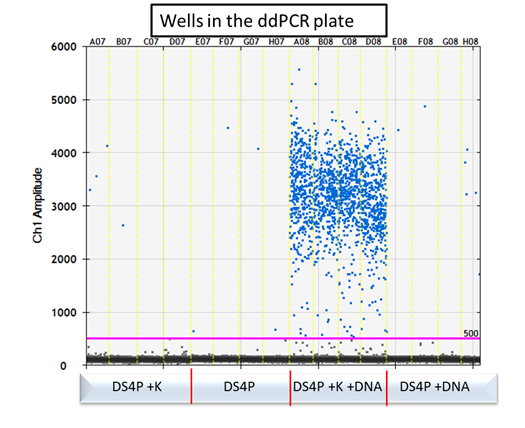
\includegraphics[max size={\textwidth}{\textheight}]{quantasoftThreshold.png}
    \caption[QuantaSoft threshold from a study]{QuantaSoft threshold in pink line from \cite{hussainThreshold}}
        \label{fig:demoQuantThreshold}
\end{figure}

The evaluation of the QuantaSoft software show satisfactory results from the food safety study of \citeA{Basanisi2020}, whereby nine pure meat samples were discriminated with 100\% diagnostic accuracy, sensitivity, and specificity. However, upon checking the authenticity of twenty commercially available meat products, twelve samples were said to contain DNA traces of other animals not declared. Among the several reasons for this high detection, \citeA{Basanisi2020} emphasizes the need for a highly sensitive and specific test at the molecular level.

Assessing the QuantaSoft software's ability to classify droplets, it was shown that for samples exhibiting a substantial amount of intermediate fluorescence, the system fails to determine a threshold (outputs "No call"). This was the case in the bacteria study of \shortciteA{Dreo2014}, that were ran on very high concentrations. In the case of low bacteria concentrations, droplets near the negative droplets were classified as positives. Similarly, \shortciteA{Witte2016} has observed around 10\% positive count differences between low and high threshold settings using the same data. The heavy presence of rain in their assay prevented a clear threshold value.  Both these studies noted that the QuantaSoft software requires a well-optimized assay with good discrimination of positive and negative droplets for its threshold to be reliable. 


\subsection{Manual Global Threshold (MTg)}
\label{sec:manthreshold}
As opposed to the automatic threshold, \citeA{Dreo2014} proposes setting a manual global threshold (MTg) determined by no template control (NTC) samples. This takes into consideration that individual assays behave differently, and could require expert intervention. As a standard approach, the threshold for a well-optimised assay was defined as the NTC mean + 6 standard deviations; on the other hand, a noisy assay had its threshold set above the highest value in NTC samples. It is expected in the latter case that the sensitivity would be lower, due to its high threshold. However, the paper claims that this resulted in high analytical sensitivity for that assay. A major disadvantage in this approach is the lack of a clear definition or guideline in setting the MTg; this consequently will cause reproducibility issues for succeeding experiments and external researchers.


\subsection{definetherain}
\label{sec:knn}
Based on the research papers curated by \citeA{Peterson:2009}, K-nearest-neighbor (KNN) is a unsupervised clustering approach that should be among the first methods considered for data with little to no information about its distribution. This clustering method operates on the chosen distance measure — commonly the Euclidean distance — between the observations. Due to its simplicity, data from various fields have applied KNN such as in a movie recommendation system \cite{Ahuja2019}, climate classification \cite{Shi2020}, breast cancer diagnostics \cite{Mittal2019}, among others.

The positive and negative droplet classification can be framed as a clustering problem. An open-source tool developed by \shortciteA{Jones2014}, called definetherain, utilizes the KNN algorithm in identifying rain droplets. According to their research, they claim that definetherain is accurate in estimating assays with low template numbers, which is particularly applicable in research fields such as the HIV-1 cure research. definetherain follows these steps for classification:
\begin{enumerate}
    \item Setup a positive control sample of known input copy numbers. 
    \item Cluster the droplets using kNN with \(k=2\). The cluster on the left is the negative cluster, and on the right is the positive cluster. 
    \item Observations between the range of the negative cluster's mean + 3 standard deviations and the positive cluster's mean - 3 standard deviations are classified as rain.
    \item Rain droplets are not included in the final calculation of the concentration estimate.
\end{enumerate}

\begin{figure}[h]
    \centering
    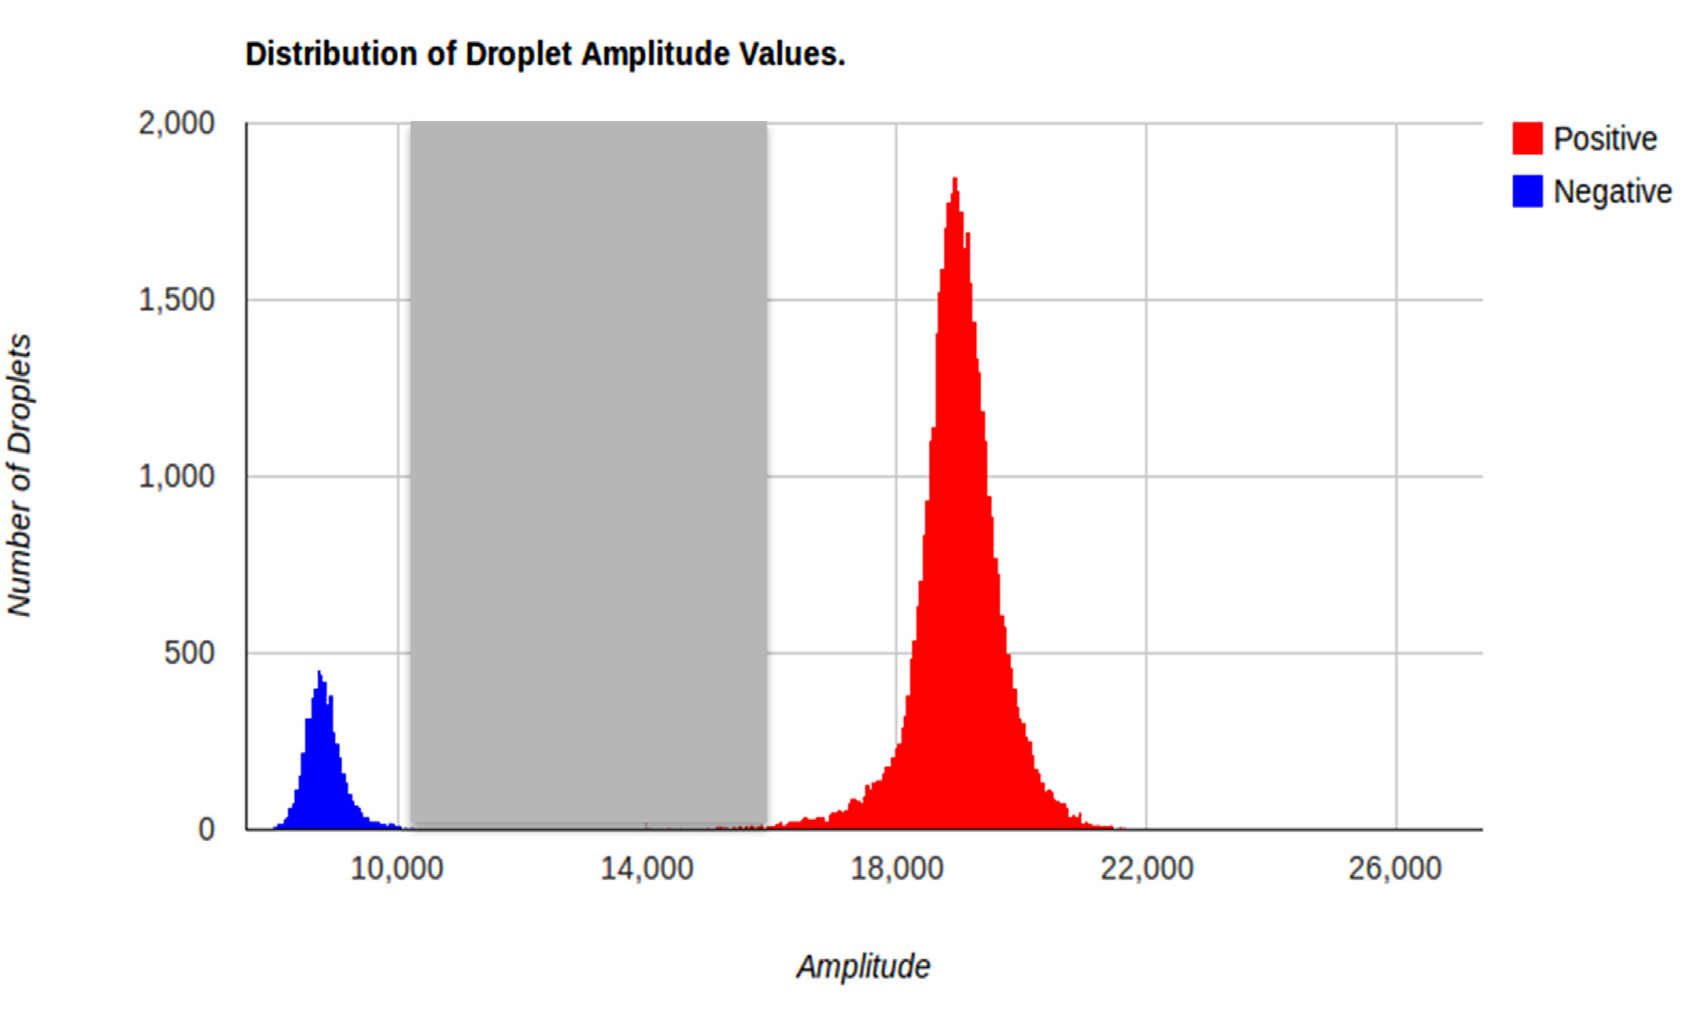
\includegraphics[max size={\textwidth}{\textheight}]{dtrsample.png}
    \caption[Determined thresholds calculated by definetherain]{Determined thresholds calculated by definetherain, reprinted from \cite{jonesThreshold}}
        \label{fig:dtrsample}
\end{figure}

Unlike the other methods discussed here, this tool produces two cutoff values — one for each cluster. The droplets falling between these two values are classified as rain. These cutoff values are solely dependent on the control sample. The disadvantages of the use of a constant threshold for the succeeding target samples is that 1) the control has to be representative of the target, otherwise, concentration estimates would be biased; and 2) the baseline shift of the fluorescence populations are not taken into consideration.

\subsection{Cloudy}
\label{sec:peakdetectionkde}
The research work of \citeA{Lievens2016} has been well cited for its definition of the performance criteria for dPCR assays as well as optimization parameters. The quantification method used in their experiments was available as a supplementary file named "S3\_file.R", which is captioned as their main function to categorize droplets and quantify the concentration. Inside this R code is a function named cloudy. Although "cloudy" was not mentioned in their paper, their algorithm will be refered here as cloudy. 

The cloudy algorithm first determines the fluorescence populations using density peaks, then iteratively estimates the parameters of each population. The droplet categorization depends on its standard deviation distance from a population's mean estimate. The following list summarizes the cloudy algorithm:
\begin{enumerate}
    \item The Guassian kernel density of the fluorescence is estimated with a minimum bandwith of 50
    \item Density peaks are identified using a sliding window approach. The subsequent steps will differ according to if one, two, or more than three peaks were found.  But generally, the proceeding steps are followed.
    \item For each population found through the peaks, its location and spread is initially estimated using the median \(\hat{\mu}\) and \(\hat{\sigma}\). Assuming normality, the latter is estimated as half the peak width at 60-65\% of its maximum height.
    \item Refine the estimates using a reiterative method, first initialized with \(a=4\).
    \item Re-estimate \(\hat{\mu}\) and \(\hat{\sigma}\) using only the observations within \(\hat{\mu} \pm (a \cdot \hat{\sigma})\).
    \item Recalculate \(a=4.55 + 0.35 \cdot log(k) + 0.045 \cdot log(k)^2\); where \(k\) is the kurtosis of the distribution
    \item Repeat steps 5-6 until stabilization.
    \item After stabilizing the estimates for all the population, the last step is different when either including or excluding rain in the final categorization. 
    \begin{enumerate}
        \item If rain is included as a category, observations within \(\hat{\mu} \pm (a \cdot \hat{\sigma})\) are then classified as members of that population; observations not falling within any population are classified as rain.
        \item If rain categorization is not of interest, then a threshold \(\theta=\hat{\mu_n} + 1.5 \cdot a_n + \hat{\sigma_n}\) is calculated; where \(n\) is a population.  
    \end{enumerate}

\end{enumerate}

In summary, the cloudy algorithm uses the Gaussian kernel density to detect peaks, which are then considered as populations. Population parameters are then estimated iteratively until convergence. It is worth noting that in its iterative step for estimating the population parameter (step 6), the formula for re-calculating \(a\) is based on the analysis of their in-house data, and should be used with caution when implementing for other unobserved nucleic acid targets. After determining the final population parameters, a range or a single threshold is then calculated for classifying droplets as positive, negative, or optionally, rain. However, the rain classification rule in step 8(a) poses a problem for fluorescence densities that are heavily skewed. \figref{fig:skeweddist} left panel reveals the distribution of negative droplets to be heavily skewed to the right, thereby causing their exclusion to be labeled as negative due to the symmetry of the categorization rule (right panel).

\begin{figure}[h]
    \centering
    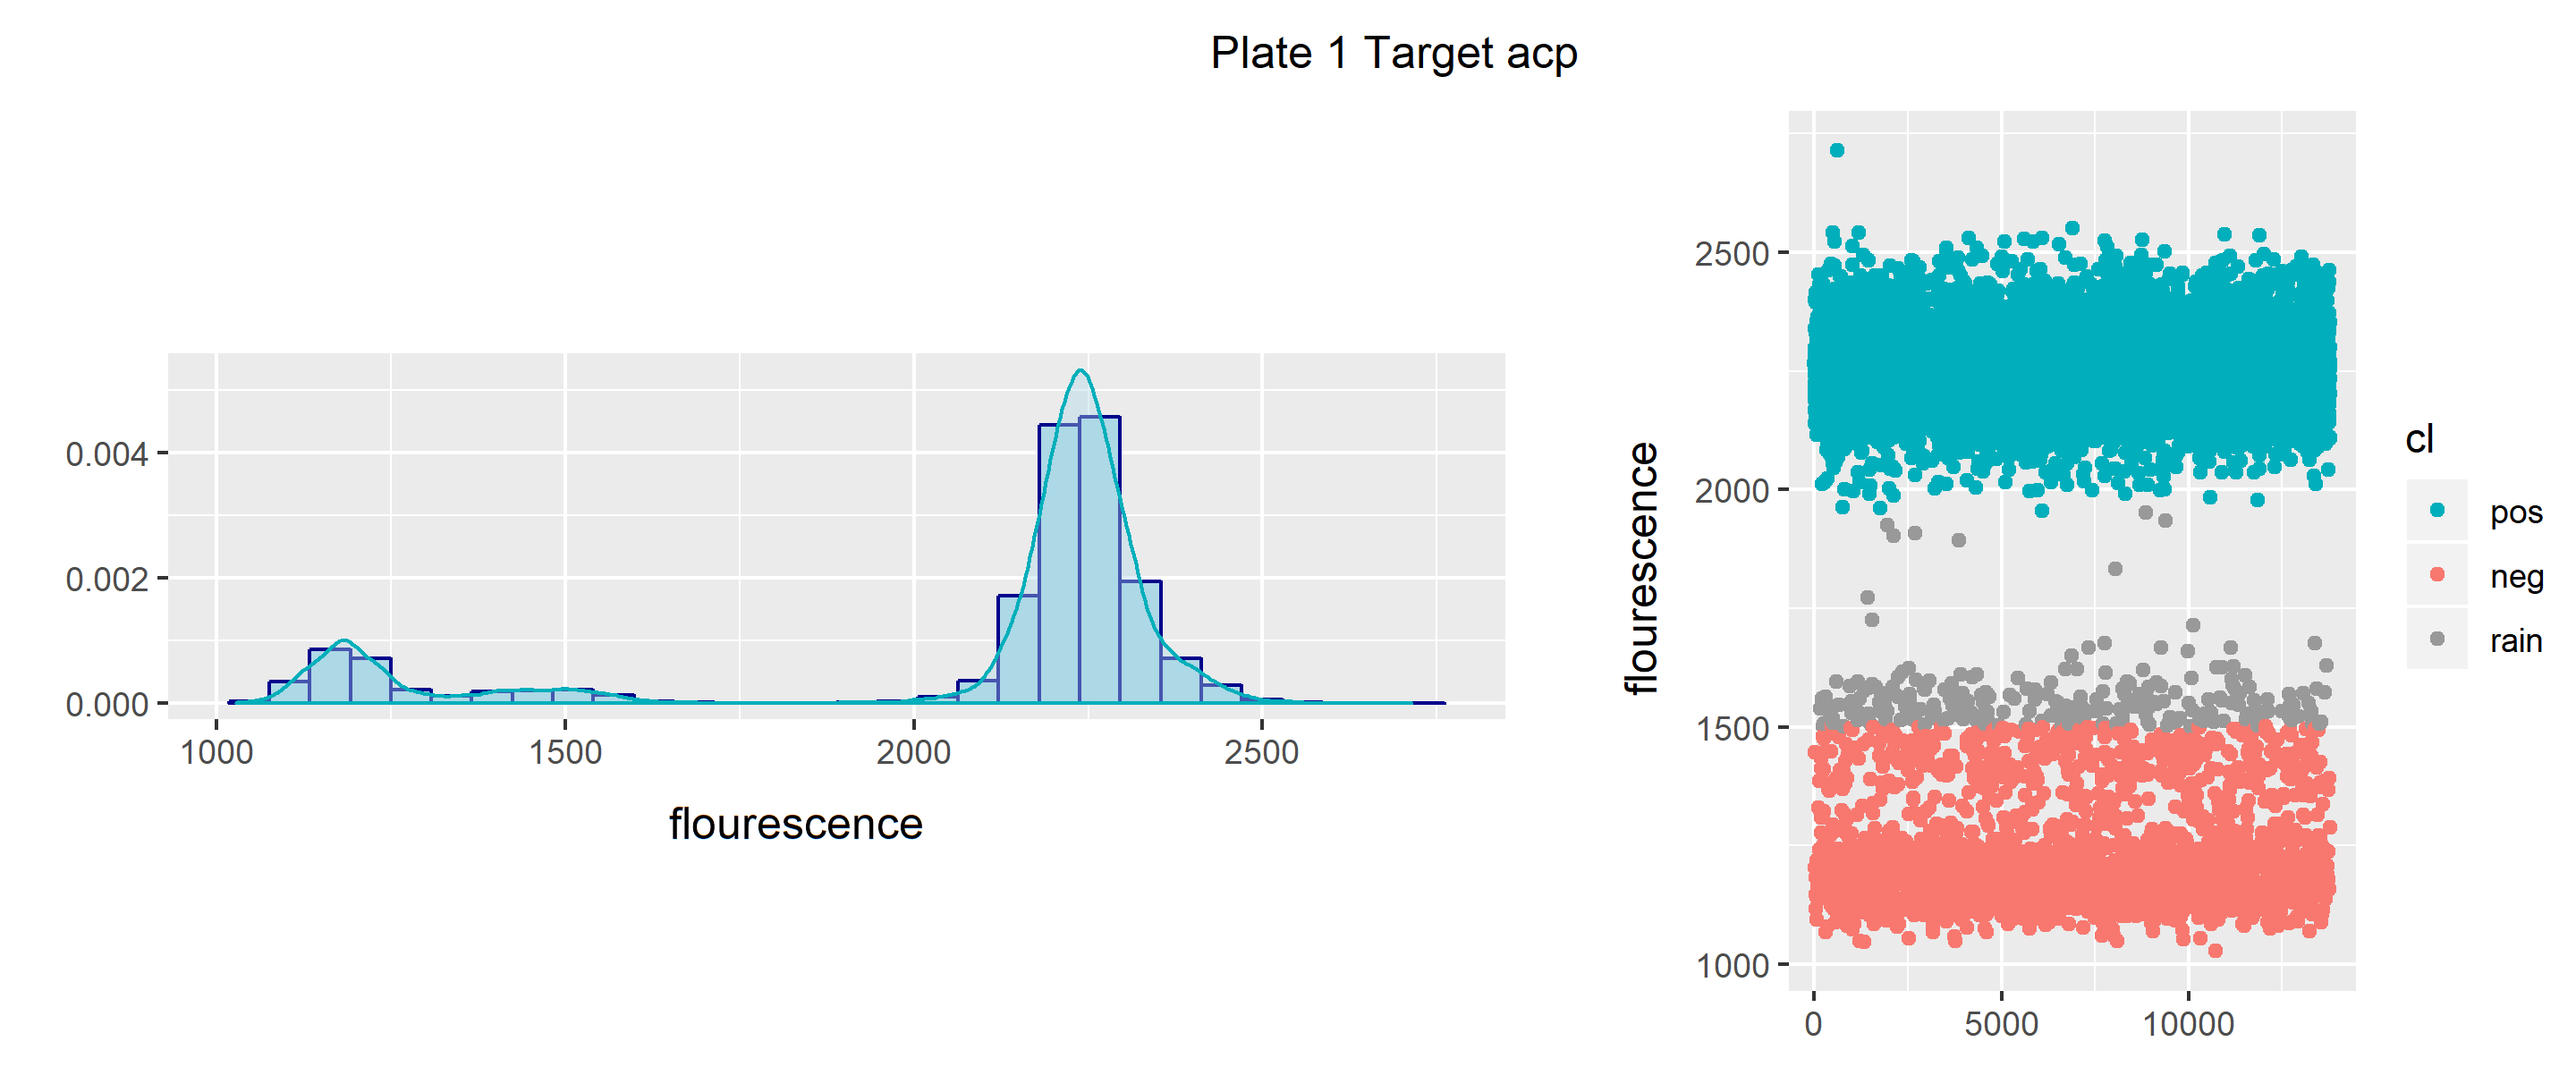
\includegraphics[max size={\textwidth}{\textheight}]{skeweddist.png}
    \caption[Fluorescence distribution of DNA target acp]{One replicate of the DNA target acp Plate 1 from \citeA{Lievens2016} dataset. Left panel shows the fluorescence densities. Right panel is the result of droplet categorization using cloudy}
        \label{fig:skeweddist}
\end{figure}

It is noted that the context of the threshold setting here is based on in-house data, and may not necessarily conclude as a classifier for external experiments. In their study, the cloudy algorithm was able to produce estimates for differing PCR experimental factors, such as sonication, PCR enhancers, annealing conditions, and number of cycles, to achieve optimization or diminishing rain droplets for dPCR experiments.


\subsection{Umbrella}
\label{sec:nonparamdensityest}

As opposed to the distance-based clustering in Section \ref{sec:knn}, a probabilistic approach is achieved with model-based clustering. According to \citeA{Mcnicholas2016}, a finite mixture model is a sum of weighted density components. This mixture model has to be appropriate such that its parameters are flexible for fitting the characteristics of the data. In this approach, each unimodal density component are defined as a cluster; and each observation has a calculated probability of it belonging to a cluster. 

The use of mixture models for clustering has been found to have many applications. In an electricity usage profiling study, \citeA{Li2018_gmm} noticed several elongated ellipses in the scatterplot of electricity usage data, urging the use of Gaussian components for their mixture model. In another example, \cite{Choy2017} performed image segmentation using the generalized Gaussian density model, where each cluster formed is interpreted as an object. Their algorithm was able to segment objects such as a starfish, cat, or tree in photographs. Additionally, using genetic data, \citeA{Li2018_mRna} discovered a potential differentially-variable microRNA (miRNA) not yet reported in literature, upon fitting a three-component multivariate normal distribution to miRNA expression levels. The assumption of the Gaussian component distributions are common in model-based clustering; however, in the succeeding texts, dPCR droplet fluorescence populations are claimed to be not normally distributed. 

In the application dPCR, \shortciteA{Jacobs2017} developed Umbrella, a model-based clustering for dPCR droplets using nonparametric density estimation (https://github.com/statOmics/umbrella). Umbrella requires a set of representative NTC sample(s), the procedure then follows a series of assumptions and estimations in deriving the final estimated concentration. An oversimplification of the Umbrella procedure are as follows:
\begin{enumerate}
    \item The NTC distribution \(f_0(x)\) is assumed to follow a unimodal distribution. The location and variation is estimated by the mode and mean of absolute deviation (MAD), respectively.
    \item The fluorescence intensitities \(x\) observed in partitions of a target partition set \(A\) is assumed to have a mixture density 
    \[f_A(x) = p_{0,A}f_{0,A}(x) + (1-p_{0,A})f_{1,A}(x)\]
    \begin{itemize}
        \item \(p_{0,A}\) = proportion of negative partitions
        \item \(f_{0,A}(x)\) = densities of the partitions without target copy (null component of the target partition set \(A\))
        \item \((1-p_{0,A})\) = proportion of positive partitions
        \item \(f_{1,A}(x)\) = densities of the partitions with target copy
    \end{itemize}
    \item Begin estimating the parameters by first aligning the modes of  the null component of \(f_A(x)\) and the NTC reference \(f_0(x)\).
    \item Discretize the aligned distributions by generating a histogram with the same bins.
    \item The bin counts of the aligned distribution are modeled using a Poisson regression model, resulting in estimates for \(\hat{p}_{0,A}\),\(\hat{f_{0}}(x)\), and \(\hat{f_{A}}(x)\).
    \item The posterior probability that partition \(i\) is void of the NA target with fluorescence intensity \(x_i\) of partition set \(A\), \(\hat{p_{0,A}}\), can be defined from the estimated \(\hat{p}_{0,A}\) from the previous step as
    \[ \hat{p}_{i,0,A}=\hat{p}_{0,A}\left(\begin{array}{c}\hat{f}_{0,A}(x_i)\\ \hat{f}_{A}(x_i)\end{array}\right) \]
    \item The Umbrella threshold estimator is then determined by the estimated \(\hat{p}_{i,0,A}\). For intensity value \(i\), the interpretation of the posterior probabilities are 
    \begin{itemize}
        \item \(\hat{p}_{i,0,A} > 80\%\) are considered negative partitions with a probability of \(\leq20\%\) to be false negatives
        \item \(\hat{p}_{i,0,A} < 5\%\) are considered positive partitions with a probability of \(\leq5\%\) to be false positives
        \item \(5\% \leq \hat{p}_{i,0,A} \leq 80\%\) are considered as rain
    \end{itemize}
\end{enumerate}

The mode and MAD, which estimates the location and spread for the null NTC distribution, \(f_{0}(x)\), are chosen due to its robustness and insensitivity to skewed tails. Only observations within 10 deviations of the mode are included for the null model.

Following the assumption of a mixture density in step 2, unlike most model-based clustering algorithms, Umbrella does not assume normal densities for \(f_{1,A}(x)\) and \(f_{0,A}(x)\), the partitions with and without the nucleic acid target, respectively. This is due to the exhibition of dPCR fluorescence intensities to be non-normal, as clusters tend to have heavy tails to the left or to the right. The solution for this is the use of non-parametric density estimation in step 3.

After estimating all the components in the mixture model from steps 3 - 5, the component of interest \(\hat{p_{0,A}}\) is then used to determine \(\hat{p}_{i,0,A}\) in step 6. Finally, this is used as the basis for Umbrella threshold estimator in step 7. It is warned that Umbrella may not be precise in detection experiments for low copy samples, as classifying individual samples is not the strength of this method.

\subsection{ddpcRquant}
\label{sec:ddpcrquant}
The ddpcRquant determines a threshold for negative droplet fluorescence based on extreme value theory. It is available as an R library developed by Trypsteen et. al (2015). The extreme value theory assumes that the maxima distribution of large samples are distributed as a generalized extreme value (GEV), regardless of the original value's distribution. Hence, the extreme value theory is considered as asymptotically nonparametric provided that samples are sufficiently large. Applying this theory in dPCR droplet classification, an extreme value percentile of the merged NTC samples are used to calculate the threshold. The summarized steps of ddpcRquant are described below :
\begin{enumerate}
    \item The required NTC sample inputs are baseline corrected. This is done subtracting the fluorescence intensities of each sample by the Robertson-Cryer estimated mode.
    \item The fluorescence of all NTC samples are merged, and then randomly assigned to equally sized \(k\) groups, 
    \item Using the maxima of all \(k\) groups, the generalized extreme value distribution is fitted by maximum likelihood.
    \item The tentative threshold is then the 0.995 percentile of this distribution.
    \item The final threshold is the average of all thresholds upon 100 repeats of steps 2-4.
    \item To correct for the baseline of target samples, each sample is subtracted by its fluorescence mode below a cutoff \(c\) — calculated as the average of the NTC modes plus the final threshold.
    \item Finally, to calculated the target concentration, negative and positive droplets are separated using the final threshold from the baseline-corrected target samples. 
\end{enumerate}

The advantages of ddpcRquant are that it doesn't assume any distribution of the droplet fluorescence, corrects for baseline shifts.  In calculating the target concentration, it does not discard any droplet as it states can underestimate the true concentration.

According to the authors' evaluation, ddpcRquant is superior to QuantaSoft in regards to having less false positive counts in the NTC samples, as a consequence, QuantaSoft concentration estimates are generally higher as it identifies more positive droplets. The reason was found to be that Quantasoft places its threshold too close to the negative droplet population, and may be caused by no baseline correction between NTC and target samples, and by its assumption of NTC being normally distributed without fitting experiments. Additionally, QuantaSoft fails to quantify concentration in some samples that result in "No call" outputs.


\section{Expectation-Maximization (EM) Clustering}
\label{sec:emclustering}

Recall from Section \ref{sec:nonparamdensityest}, model-based clustering refers to fitting a finite mixture model given the data set \(X\); then the cluster membership of observation \(x_i\) is determined by the highest probability of it belonging to a density component. Building the mixture model \(f(x|\Theta)\) requires the determination of 1) \(G\) — the number of mixture components (clusters) and 2) \(f_g(x|\theta_g)\) — the distribution assumed to be followed by the mixture component \(g\). 

A common method for determining \(G\) is by selecting the model with the lowest Bayesian Information Criterion (BIC) amongst the proposed \(G\)-component mixture models. As mentioned in the model-based clustering examples in Section \ref{sec:nonparamdensityest}, the mixture components are frequently assumed to follow a Gaussian distribution, and is also known as Gaussian Mixture Model (GMM). Although popular, GMMs poorly fit the data that exhibit skewness and different levels of kurtosis, consequently leading to overestimation on the number of clusters \cite{Dang2019}. Alternatively, the following distributions can better generalize these kinds of data: multivariate \(t\), skewed-\(t\), multivariate power exponential, variance-gamma, generalized hyperbolic, etc. Unlike Gaussian, these component models are flexible for data with varying tail weight, peakedness, and skewness.

After determining the distribution of \(G\) mixture components, the next problem is on how to estimate its corresponding parameter set \(\Theta*\). Expectation-Maximization (EM), a well-known parameter estimation algorithm, is an iterative procedure that maximizes the likelihood of the parameters given the observed data \cite{Garriga2016}. In the EM procedure, the parameter set is initially guessed and is re-estimated in every iteration of the E-step and M-step, until the parameter set reaches convergence. E-step computes the likelihood weight, or the posterior probability, of each data point \(x_i\) belonging to a component \(g\). M-step re-estimates new parameters that maximize the likelihood of these weights for each component. The result of EM guarantees to reach a local maximum for parametric distributions. The direct application of using the final EM posterior probabilities in assigning data points to groups is called EM Clustering (EMC) \cite{Garriga2016}. 

For dPCR droplets classification, since the groups of interest are the positive and negative droplets, a two-component mixture model suffices. However, observations of dPCR data reveals that three or more populations may form; in this case, \(G\) will have to be determined. Additionally, there is room for research in identifying the fluorescence intensity distribution that will fit the characteristics of the positive/negative groups. Since heavy tails are observed in fluorescence densities in \figref{fig:skeweddist}, distributions have to be explored that may best fit the data. 


\section{Performance Evaluation for Quantification Estimates}
\label{sec:ch2_perfeval_estimates}
               %-- includes LaTeX source file for Chapter 2: Review of Related Literature
                                  %-- your job: **EDIT THIS FILE** to indicate your review of related literature 

\chapter{Theoretical Framework}
\label{sec:theoreticalframework} 


\section{EM Clustering}
\label{sec:modelbased_ch3}

\subsection{Model-based clustering}
\label{sec:gcomponentmixturedensity}

\subsection{G-component Finite Mixture Density}
\label{sec:gcomponentmixturedensity}

\subsection{Expectation Maximization}
\label{sec:em}

\section{Performance Evaluation}
\label{sec:emclustering_ch3}
               %-- includes LaTeX source file for Chapter 3: Research Methodology
                                  %-- your job: **EDIT THIS FILE** to indicate your research methodology
                                  
\chapter{Methodology}
\label{sec:methodology} 

\section{Data}
\label{sec:data}

\subsection{Rain Experiment Dataset}
\label{sec:experimentdataset}

\subsubsection{Plate 2 - Primer and Probe Concentration Gradient}
\label{sec:plate2}

\subsubsection{Plate 4 - PCR Enhancers Experiment}
\label{sec:plate4}

\subsubsection{Plate 5 - Cycle Gradient}
\label{sec:plate5}

\subsubsection{Plate 6 - Sonication Gradient}
\label{sec:plate6}

\subsubsection{Plate 7 - Annealing Temperature Gradient}
\label{sec:plate7}

\subsection{DNA Quantification Dataset}
\label{sec:quantificationdataset}

\subsubsection{Plate 3 - Rain Dilution Series}
\label{sec:plate3}

\subsubsection{Albumin}
\label{sec:albumin}

\section{Model Fitting and Classification}
\label{sec:modelfitting}

\section{Performance Evaluation}
\label{sec:performanceeval}
               %-- includes LaTeX source file for Chapter 3: Research Methodology
%-- your job: **EDIT THIS FILE** to indicate your research methodology


\appendix                         %-- used to specify appendices
%%%%%%%%%%%%%%%%%%%%%%%%%%%%%%%%%%%%%%%%%%%%%%%%%%%%%%%%%%%%%%%%%%%%%%%%%%%%%%%%%%%%%%%%%%%%%%%%%%%%%%
%
%   Filename    : appendix_A.tex 
%
%   Description : This file is one of the appendices. 
%                 
%%%%%%%%%%%%%%%%%%%%%%%%%%%%%%%%%%%%%%%%%%%%%%%%%%%%%%%%%%%%%%%%%%%%%%%%%%%%%%%%%%%%%%%%%%%%%%%%%%%%%%

\chapter{Diagrams and Other Documentation Tools}
\label{sec:appendixa}


This appendix may consist of proposed architectural design, algorithms, scientific formula for 
MSCS and Data Flow Diagrams, Fishbone for MSIT.


              %-- includes LaTeX source file for Appendix A
                                                 %-- your job: **CREATE/EDIT** your own source file for the appendices
%%%%%%%%%%%%%%%%%%%%%%%%%%%%%%%%%%%%%%%%%%%%%%%%%%%%%%%%%%%%%%%%%%%%%%%%%%%%%%%%%%%%%%%%%%%%%%%%%%%%%%
%
%   Filename    : appendix_B.tex 
%
%   Description : This file will contain one of your appendices.
%                 
%%%%%%%%%%%%%%%%%%%%%%%%%%%%%%%%%%%%%%%%%%%%%%%%%%%%%%%%%%%%%%%%%%%%%%%%%%%%%%%%%%%%%%%%%%%%%%%%%%%%%%

\chapter{Theoretical and/or Conceptual Framework}
\label{sec:appendixb}

Discusses the basic framework/foundation the thesis is based on. This section is normally referred to when discussing Scope and Limitations,
and Research Methodology



%%%%%%%%%%%%%%%%%%%%%%%%%%%%%%%%%%%%%%%%%%%%%%%%%%%%%%%%%%%%%%%%%%%%%%%%%%%%%%%%%%%%%%%%%%%%%%%%%%%%%%
%
%   Filename    : appendix_C.tex
%
%   Description : This file will contain information about your Resource Persons
%                 
%%%%%%%%%%%%%%%%%%%%%%%%%%%%%%%%%%%%%%%%%%%%%%%%%%%%%%%%%%%%%%%%%%%%%%%%%%%%%%%%%%%%%%%%%%%%%%%%%%%%%%

\chapter{Resource Persons}
\label{sec:appendixc}

%
%  Indicate your resource persons here:
%
%	<full name and title, e.g., Dr. Juan de la Cruz>
%	<profession, e.g., faculty>
%	<department, e.g., College of Computer Studies>
%	<name of institution, e.g., De La Salle University>
%	<e-mail address>
%
%

%
%  the following shows 3 examples, replace entries with your own
%
\newcommand{\resperson}[4]{\textbf{#1} \\ #2 \\ #3 \\ \url{#4}\vspace{0.5em}\\}

\resperson{Dr. Firstname1 Lastname1}{Adviser}{CCS\\De La Salle University-Manila}{emailaddr@dlsu.edu.ph}
\resperson{Mr. Firstname2 Lastname2}{Role2}{Affiliation2}{emailaddr2@domain.com}
\resperson{Ms. Firstname3 Lastname3}{Role3}{Affiliation3}{emailaddr3@domain.net}




%\bibliographystyle{apacite}       %-- specified APA style for bibliograpy
                                  %-- more details about APA style citation can be found in www.ctan.org/tex-archive/biblio/bibtex/contrib/apacite/

                                  %-- bibliographic entries are handled via bibtex; refer to www.bibtex.org for more details


\bibliography{myreferences}       %-- the file "myreferences.bib" is a sample bibliography (bib) from SIGGRAPH 
                                  %-- your job: **CREATE/EDIT** your own bibliography file  

\end{document}

